%!TEX root = ../main.tex 

\section{Qu'est-ce qu'une impédance?}

\begin{frame}{Warning - Attention}
    \begin{tikzpicture}
    
    \draw (0, 0) node[inner sep=0] {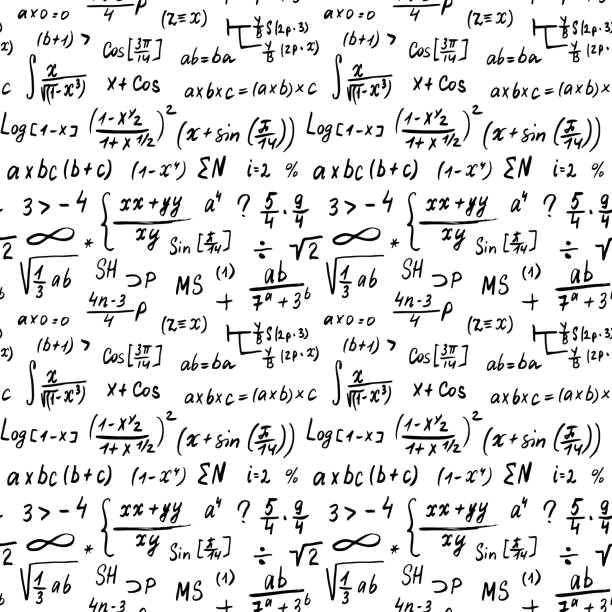
\includegraphics[width=\textwidth]{pictures/background/complex-maths.png}};
    \draw (0, 3) node[text width=20em] {
        \begin{center}
             \begin{beamercolorbox}[sep=6pt,center,shadow=true,rounded=true]{title}
             \large{La section suivante contient des\\
             \textbf{\textit{équations mathématiques}}}
             \end{beamercolorbox}
        \end{center}
     };
    \end{tikzpicture}
\end{frame}

\begin{frame}{Impédance - Relation des réactances et résistances}
    \begin{columns}
        \begin{column}{0.5\textwidth}
            \begin{itemize}
                \item Dénoté $Z$, en $\Omega$
                \item Résistance électrique à une certaine fréquence
                \item Composé de:
                \begin{itemize}
                    \item Résistance ($R$)
                    \item Réactance Inductive ($X_L$)
                    \item Réactance Capacitive ($X_C$)
                \end{itemize}
                \item Les réactances s'opposent sur l'axe imaginaire!
            \end{itemize}
            \par
            \begin{center}
                \Large{$V = ZI$}
            \end{center}
        \end{column}
        
        \begin{column}{0.5\textwidth}
            \begin{figure}
                \centering
                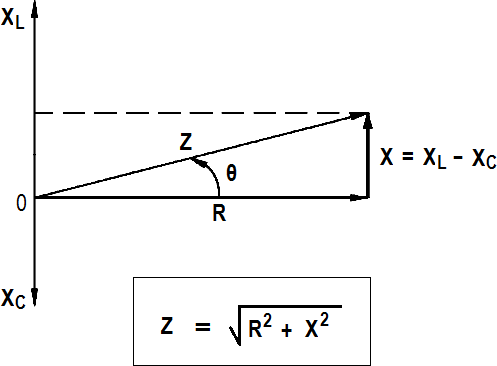
\includegraphics[width=\textwidth]{pictures/relationship-between-resistance-reactance-and-impedance.png}
            \end{figure}
        \end{column}
    \end{columns}
\end{frame}

\subsection{Réactance}
\begin{frame}{Qu'est-ce qu'une réactance?}
    \begin{itemize}
        \item Opposition à un courant alternatif
        \begin{itemize}
            \item Posé par une bobine (Réactance Inductive $X_L$)
            \item Posé par un condensateur (Réactance Capacitive $X_C$)
        \end{itemize}
        \item Pas de dissipation en chaleur!
        \item Emmagasine l'énergie et la relâche plus tard
        \begin{itemize}
            \item Champ magnétique ($X_L$)
            \item Champ électrique ($X_C$)
        \end{itemize}
        \item Entraîne un changement de phase dans un signal!
    \end{itemize}
\end{frame}

\begin{frame}{Différence de phase entre réactances}
    \begin{figure}
        \centering
        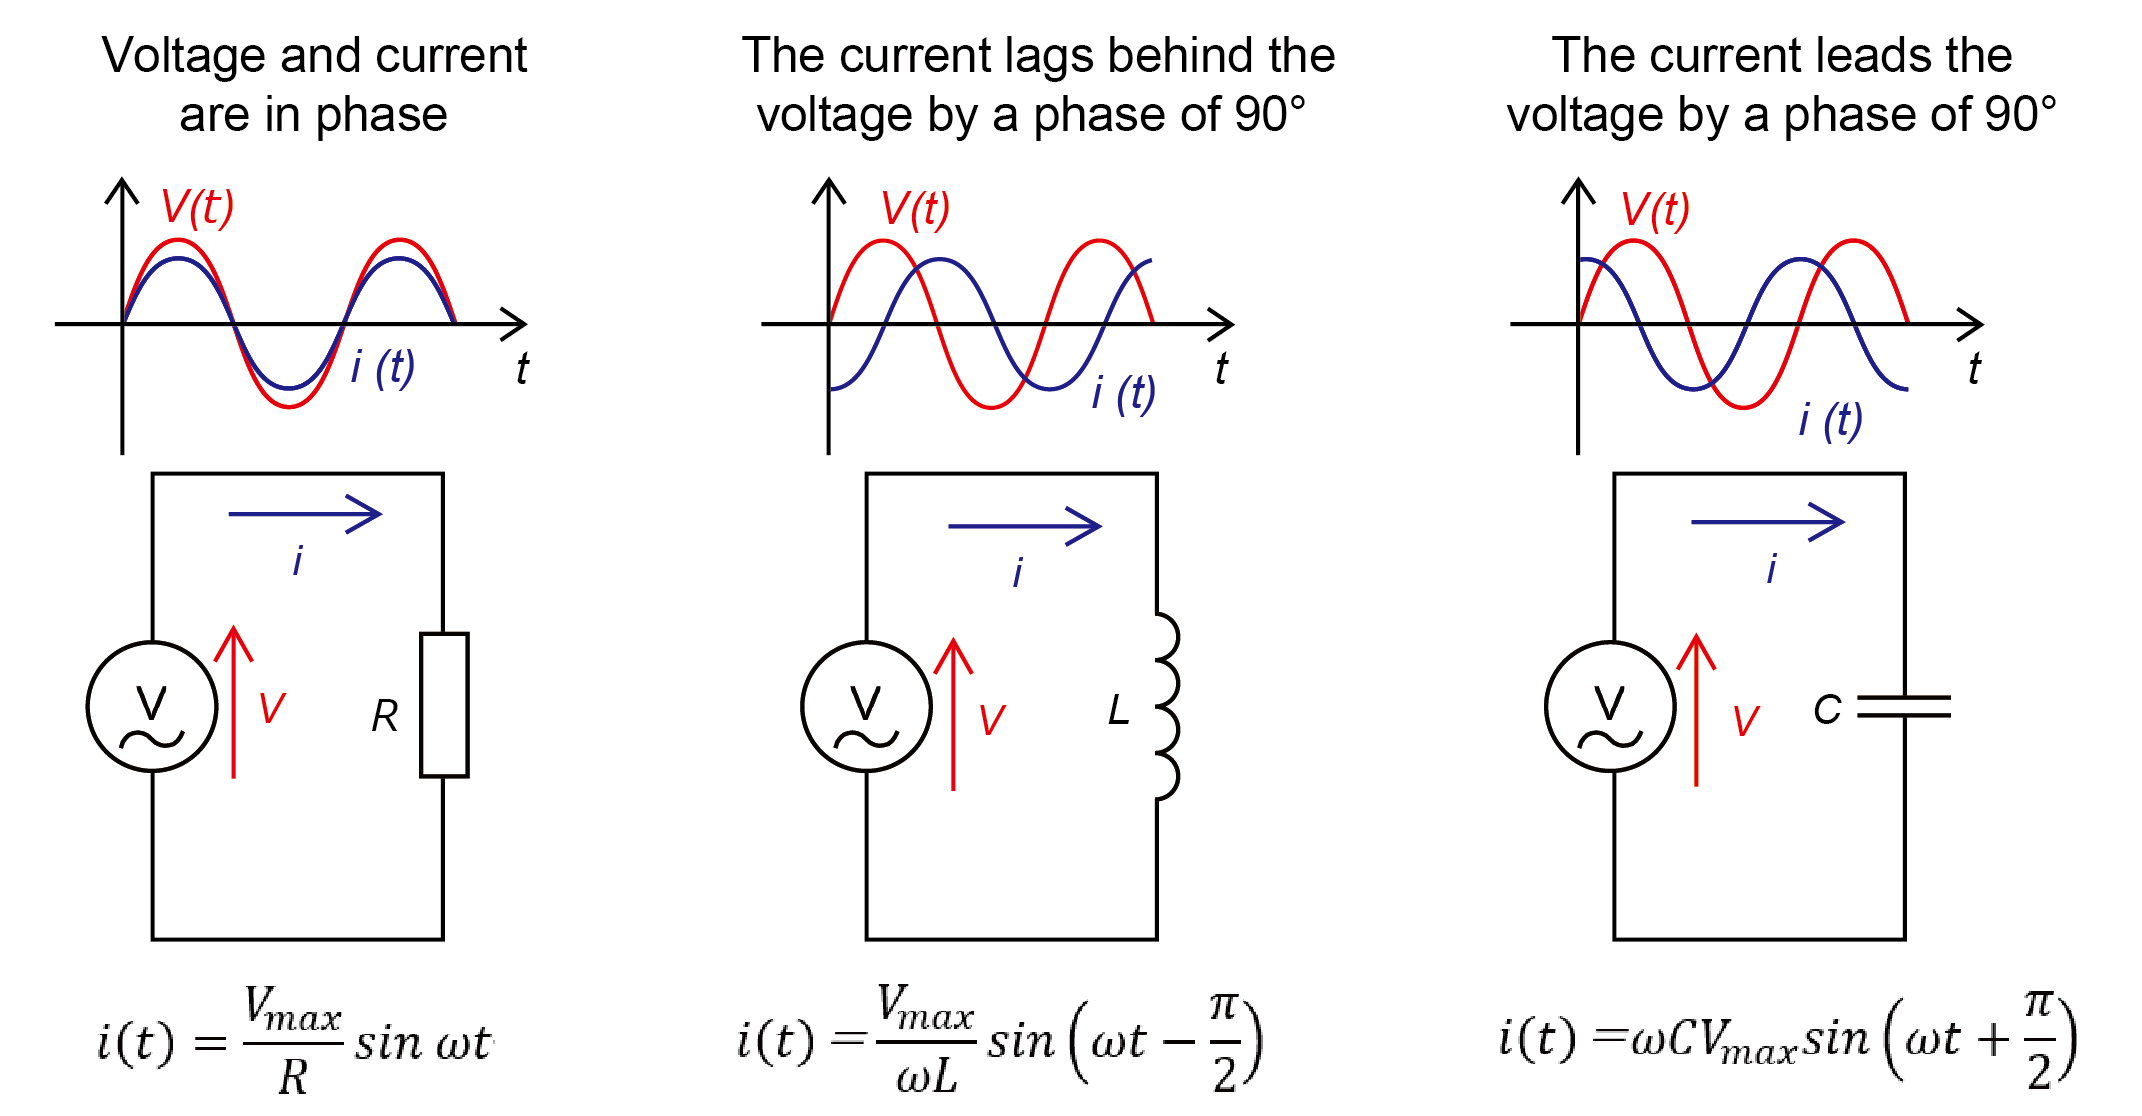
\includegraphics[width=\textwidth]{pictures/Phase_Difference_Between_Impedance_and_Current.png}
    \end{figure}
\end{frame}

\begin{frame}{Résistance}
    \begin{columns}
        \begin{column}{0.66\textwidth}
            \begin{itemize}
                \item S'oppose à tout courant
                \item Mauvais conducteur d'électricité
                \item Friction / Restriction
                \item Dissipe l'énergie en chaleur
                \item \textit{Fonctionne pareillement à toutes fréquences}
            \end{itemize}
            \par
            \begin{center}
                \Large{$V = RI$}
            \end{center}
        \end{column}
        \begin{column}{0.33\textwidth}
            \begin{figure}
                \centering
                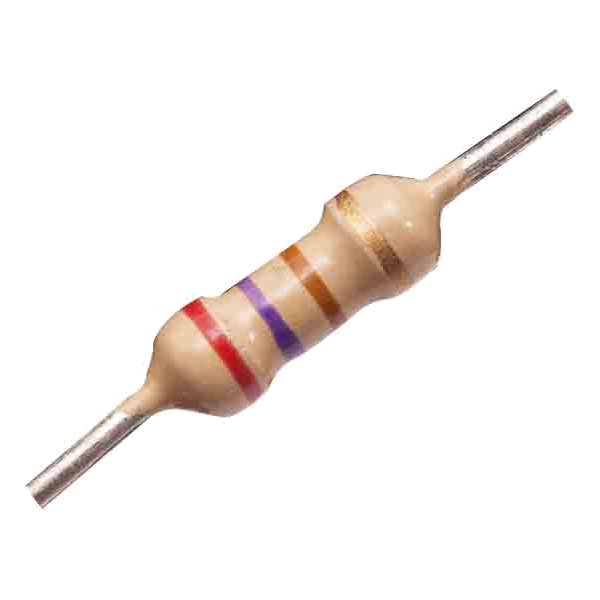
\includegraphics[width=\textwidth]{pictures/component-resistance.png}
            \end{figure}
        \end{column}
    \end{columns}
\end{frame}



% ---------------- CAPACITANCE ------------------


\iffalse


\subsection{Réactance Capacitive}
\begin{frame}{Capacitance}
    \begin{columns}
        \begin{column}{0.66\textwidth}
            \begin{itemize}
                \item S'oppose aux changements de tension
                \item Ne conduit pas en DC
                \item Emmagasine l'énergie dans les champs électriques
                \item Charges accumulées sur les plaques du condensateur
                \item \textit{Conduit plus à des fréquences plus élevées}
            \end{itemize}
            \par
            \begin{center}
                \Large{$Q = CV$}
            \end{center}
        \end{column}
        \begin{column}{0.33\textwidth}
            \begin{figure}
                \centering
                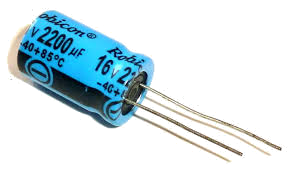
\includegraphics[width=\textwidth]{pictures/component-capacitor.png}
            \end{figure}
        \end{column}
    \end{columns}
\end{frame}

\begin{frame}{Condensateur simple}
    \begin{columns}
        \begin{column}{0.66\textwidth}
            \begin{itemize}
                \item Deux plaques espacées, avec un matériau entre les plaques
                \item Des charges s'accumulent entre les plaques
                \item Différence de potentiel entre les plaques
                \item Énergie emmagasinée dans les champs électriques
            \end{itemize}
            \par
            \Large{
            \begin{center}
                $C = \varepsilon_0 \varepsilon_r \frac{A}{d}$
            \end{center}
            }
        \end{column}

        \begin{column}{0.33\textwidth}
            \begin{figure}
                \centering
                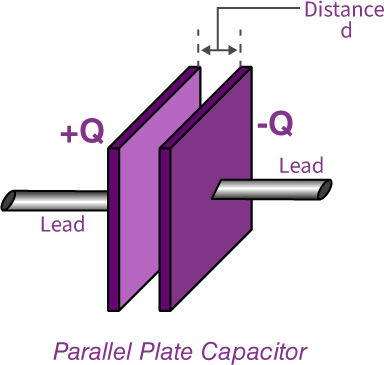
\includegraphics[width=\textwidth]{pictures/parallel-plate-capacitor.png}
            \end{figure}
        \end{column}
    \end{columns}
\end{frame}

\begin{frame}{Capacitance - Équations - Différentiation}
    \begin{columns}
        \begin{column}{0.5\textwidth}
            \begin{itemize}
                \item Quantité de Charge = Capacitance * Tension
                \item Dérivée selon le temps
                \item Ampère = Coulomb / Seconde
                \bigskip
                \item Plus de courant passe au travers du cap quand changements de tension
                \item Plus un changement est rapide ($\frac{dV}{dt}$), plus de courant passe
            \end{itemize}
        \end{column}
        \begin{column}{0.5\textwidth}
            \Large{
            \begin{center}
                $Q = CV$\\
                \vspace{10pt}
                $\frac{dQ}{dt} = C \frac{dV}{dt}$\\
                \vspace{10pt}
                $I = C \frac{dV}{dt}$\\
            \end{center}
            }
        \end{column}
    \end{columns}
\end{frame}

\begin{frame}{Capacitance - Équations - Ajout d'une fréquence}
    \begin{center}
        \Large{
            Posons $V = \sin(2 \pi t) = e^{j 2 \pi f t} = e^{j \omega t}$\\
            \vspace{15pt}
            $I = C \cdot \frac{de^{j \omega t}}{dt}$\\
            \vspace{5pt}
            $I = C j \omega \cdot e^{j \omega t}$\\
            \vspace{5pt}
            $I = C j \omega \cdot V$\\
            \vspace{20pt}
            $\dfrac{V}{I} = \dfrac{1}{C j \omega}$\\
        }
    \end{center}
\end{frame}

\begin{frame}{Capacitance - Équations - Réactance Capacitive}
    \begin{center}
        \Large{
            $X_C = \dfrac{1}{2 \pi f C}$
        }
        \vspace{15pt}
        \begin{figure}
            \centering
            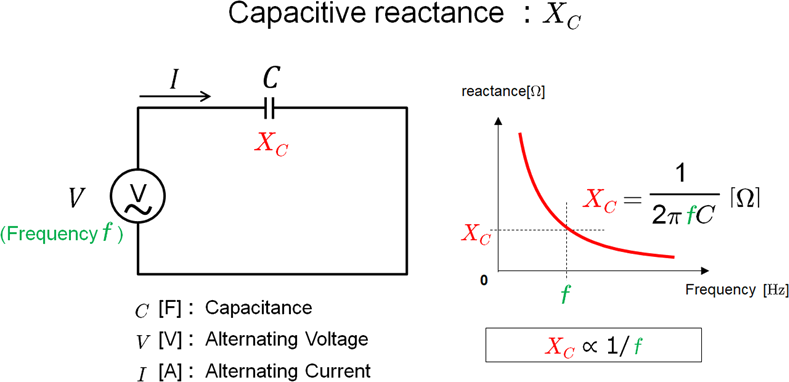
\includegraphics[width=\textwidth]{pictures/capacitive-reactance.png}
        \end{figure}
    \end{center}
\end{frame}

\begin{frame}{Capacitance - Équations - Isoler le courant}
    \begin{center}
        \Large{
            $X_C = \dfrac{1}{2 \pi f C} = \dfrac{V}{I}$\\
            \vspace{15pt}
            $I = \dfrac{V}{X_C}$\\
            \vspace{5pt}
            $I = V \cdot \omega C = V \cdot 2 \pi f C$\\
        }
    \end{center}
\end{frame}

\begin{frame}{Capacitance - Équations - Courant selon fréquence}
    \begin{center}
        \Large{
            $I = V \cdot 2 \pi f C$
        }
        \vspace{15pt}
        \begin{figure}
            \centering
            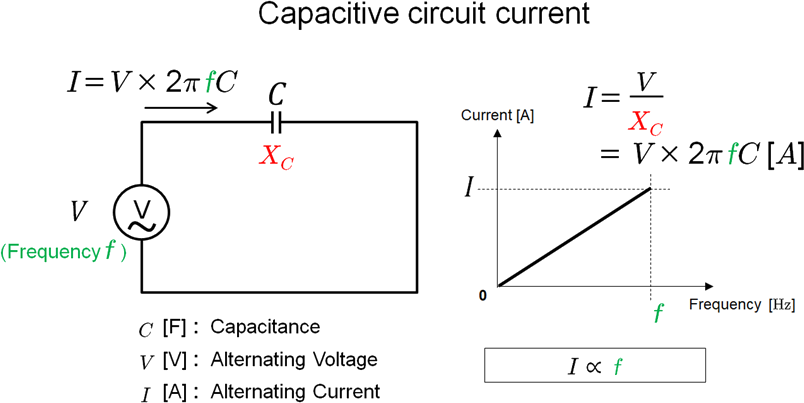
\includegraphics[width=\textwidth]{pictures/in_capacitive_reactance_the_current_is_inversely_proportional_to_the_frequency.png}
        \end{figure}
    \end{center}
\end{frame}



% ---------------- INDUCTANCE ------------------



\subsection{Réactance Inductive}
\begin{frame}{Inductance}
    \begin{columns}
        \begin{column}{0.66\textwidth}
            \begin{itemize}
                \item S'oppose aux changements de courant
                \item Conduit en DC
                \item Emmagasine l'énergie dans les champs magnétique
                \item \textit{Conduit plus à des basses fréquences}
            \end{itemize}
            \par
            \begin{center}
                \Large{$L = \dfrac{V \cdot dt}{I}$}
            \end{center}
        \end{column}
        \begin{column}{0.33\textwidth}
            \begin{figure}
                \centering
                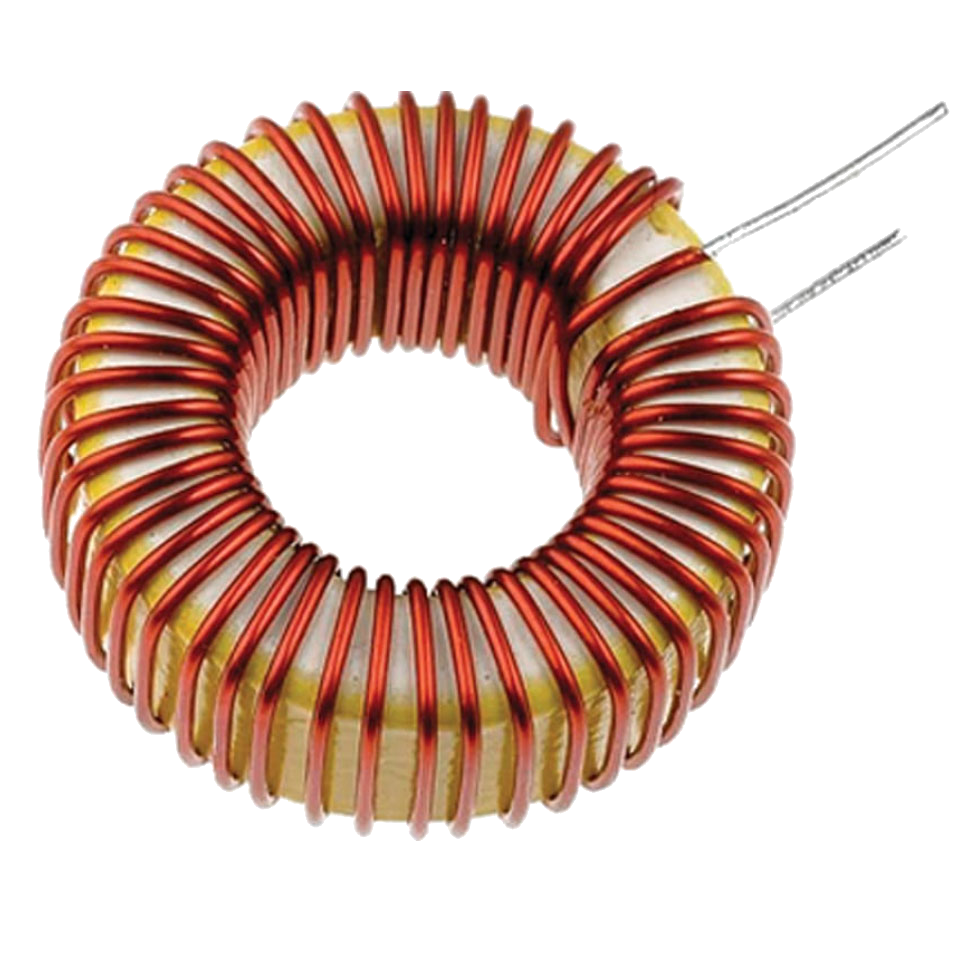
\includegraphics[width=\textwidth]{pictures/component-inductor.png}
            \end{figure}
        \end{column}
    \end{columns}
\end{frame}

\begin{frame}{Inductance simple}
    \begin{columns}
        \begin{column}{0.66\textwidth}
            \begin{itemize}
                \item Bobine de fil enroulé autour d'un matériau
                \item Flux magnétique généré par un $\frac{dI}{dt}$ dans le fil
                \item Flux magnétique fait circuler du courant dans les conducteurs autour
                \begin{itemize}
                    \item \textit{Self-induction}
                \end{itemize}
                \item Énergie emmagasinée dans les champs magnétiques
            \end{itemize}
            \par
            \Large{
            \begin{center}
                $L = \mu_0 \mu_r \dfrac{N^2A}{l}$
            \end{center}
            }
        \end{column}

        \begin{column}{0.33\textwidth}
            \begin{figure}
                \centering
                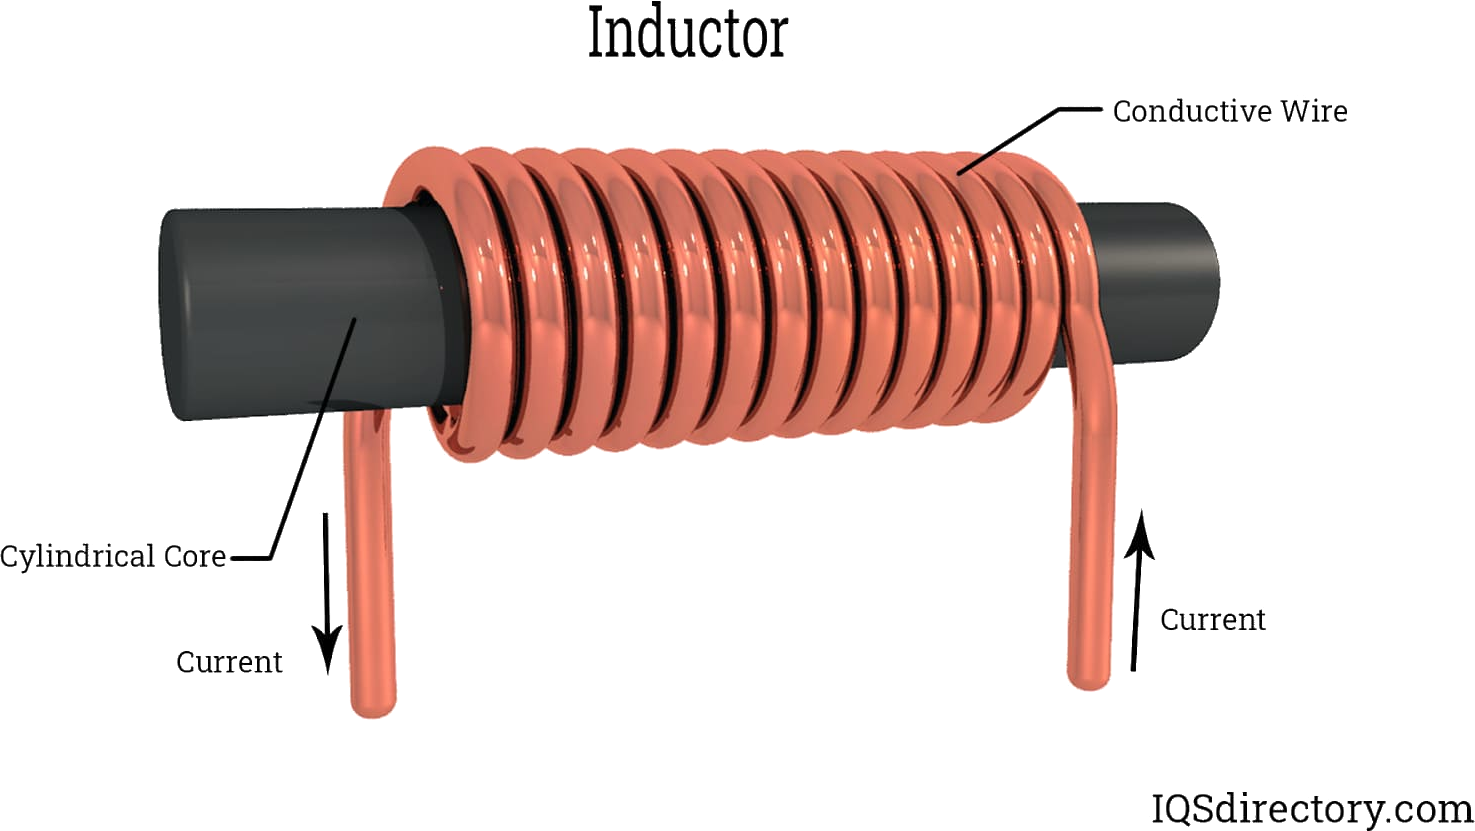
\includegraphics[width=\textwidth]{pictures/simple-inductor.png}
            \end{figure}
        \end{column}
    \end{columns}
\end{frame}

\begin{frame}{Inductance - Équations - Différentiation}
    \begin{columns}
        \begin{column}{0.5\textwidth}
            \begin{itemize}
                \item Inductance = Tension / taux de change du courant
                \item Déjà dérivée selon le temps
                \bigskip
                \item Plus de tension aux bornes de l'inductance quand changement de courant
                \item Plus un changement est rapide ($\frac{dI}{dt}$), plus la tension monte.
            \end{itemize}
        \end{column}
        \begin{column}{0.5\textwidth}
            \Large{
            \begin{center}
                $L = \dfrac{V \cdot s}{I}$\\
                \vspace{10pt}
                $V = L \frac{dI}{dt}$\\
            \end{center}
            }
        \end{column}
    \end{columns}
\end{frame}

\begin{frame}{Inductance - Équations - Ajout d'une fréquence}
    \begin{center}
        \Large{
            Posons $I = \sin(2 \pi t) = e^{j 2 \pi f t} = e^{j \omega t}$\\
            \vspace{15pt}
            $V = L \cdot \frac{de^{j \omega t}}{dt}$\\
            \vspace{5pt}
            $V = L j \omega \cdot e^{j \omega t}$\\
            \vspace{5pt}
            $V = L j \omega \cdot I$\\
            \vspace{20pt}
            $\dfrac{V}{I} = L j \omega$\\
        }
    \end{center}
\end{frame}

\begin{frame}{Inductance - Équations - Réactance Inductive}
    \begin{center}
        \Large{
            $\mathcal{X}_L = 2 \pi f L$
        }
        \vspace{15pt}
        \begin{figure}
            \centering
            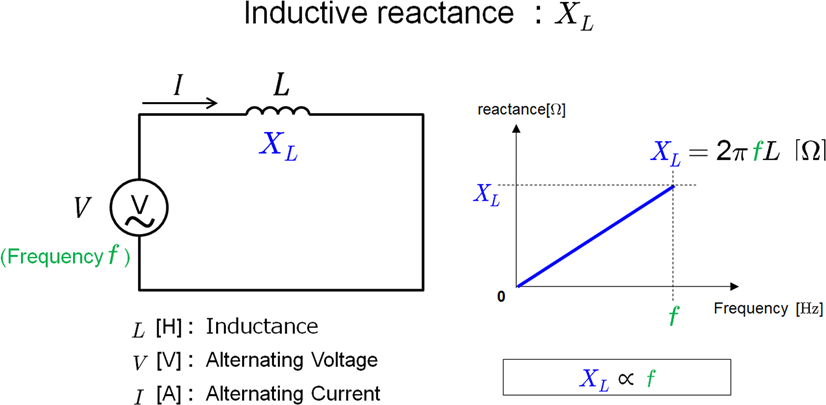
\includegraphics[width=\textwidth]{pictures/inductive-reactance.png}
        \end{figure}
    \end{center}
\end{frame}

\begin{frame}{Capacitance - Équations - Courant selon fréquence}
    \begin{center}
        \Large{
            $V = I \cdot 2 \pi f L$
        }
        \vspace{15pt}
        \begin{figure}
            \centering
            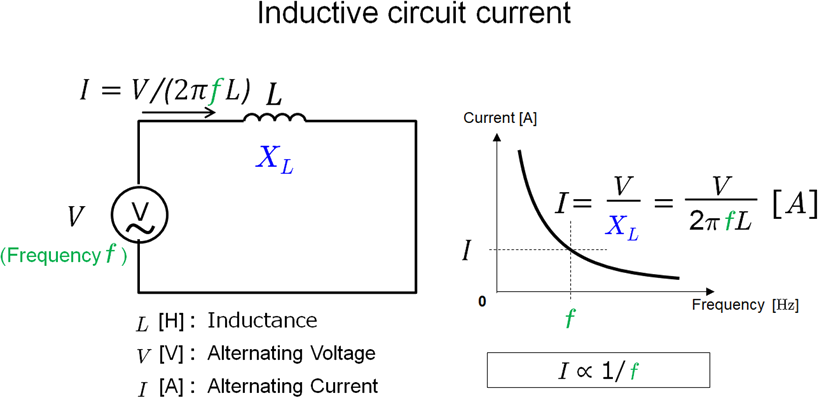
\includegraphics[width=\textwidth]{pictures/In_inductive_reactance_the_current_is_inversely_proportional_to_the_frequency.png}
        \end{figure}
    \end{center}
\end{frame}


% -------------- FILTRE ------------ %
\subsection{Filtres}
\begin{frame}{Filtre Passe-Bas RC}
    \begin{columns}
        \begin{column}{0.33\textwidth}
            \begin{center}
                $-3dB$ = $\frac{1}{2}$ puissance\\
                \vspace{10pt}
                \Large{$R = \dfrac{1}{2 \pi f C}$}
            \end{center}
        \end{column}
        
        \begin{column}{0.66\textwidth}
            \begin{figure}
                \centering
                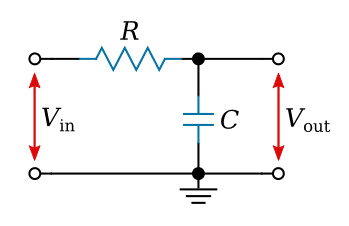
\includegraphics[width=\textwidth]{pictures/rc-low-pass-filter.png}
            \end{figure}
        \end{column}
    \end{columns}
\end{frame}

\begin{frame}{Filtre Passe-Bas RC}
    \begin{columns}
        \begin{column}{0.33\textwidth}
            \begin{center}
                \Large{$R = \dfrac{1}{2 \pi f C}$}\\
                \vspace{10pt}
                \Large{$X_C = \dfrac{1}{2 \pi f C}$}
            \end{center}
        \end{column}
        
        \begin{column}{0.66\textwidth}
            \begin{figure}
                \centering
                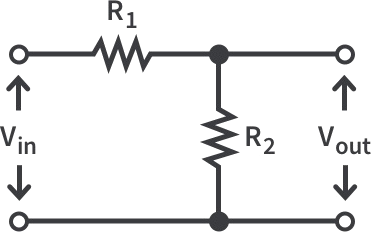
\includegraphics[width=\textwidth]{pictures/voltage-divider.png}
            \end{figure}
        \end{column}
    \end{columns}
\end{frame}


\begin{frame}{Impédance}
    \begin{columns}
        \begin{column}{0.4\textwidth}
            \begin{itemize}
                \item Amplitude défini la "résistance" réelle du circuit
                \item Phase défini le décalage du courant par rapport à la tension
                \item Power Factor
            \end{itemize}
            \par
            \vspace{10pt}
            \begin{center}
                \Large{$X_C = \dfrac{1}{2 \pi f C}$}\\
                \vspace{10pt}
                \Large{$X_L = 2 \pi f L$}
            \end{center}
        \end{column}
        
        \begin{column}{0.55\textwidth}
            \begin{figure}
                \centering
                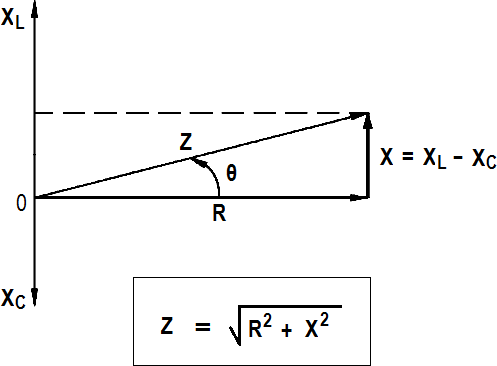
\includegraphics[width=\textwidth]{pictures/relationship-between-resistance-reactance-and-impedance.png}
            \end{figure}
        \end{column}
    \end{columns}
\end{frame}

\subsection{Ligne de transmission}
\begin{frame}{Circuit électrique de base}
    \begin{center}
    
    \resizebox{0.9\textwidth}{!}{
    \begin{circuitikz}[american voltages]
        \draw [thick]
        (0,0) to [short, *-] (10,0)
        to [R, l_=$R_{LOAD}$] (10,5)
        (0,0) to [open, v<=$V$] (0,5)
        to [short, *- ,i=$i$] (2,5)
        to [short] (10,5)
        ;
    \end{circuitikz}
    }
    \end{center}
\end{frame}

\begin{frame}{Circuit électrique - Résistance Parasite}
    \begin{center}
    
    \resizebox{0.9\textwidth}{!}{
    \begin{circuitikz}[american voltages]
        \draw [thick]
        (0,0) to [short, *-] (10,0)
        to [R, l_=$R_{LOAD}$] (10,5)
        (0,0) to [open, v<=$V$] (0,5)
        to [short, *- ,i=$i$] (2,5)
        to [R, l_=$R$] (4, 5)
        to [short] (10,5)
        ;
    \end{circuitikz}
    }
    \end{center}
\end{frame}

\begin{frame}{Circuit électrique - Capacitance Parasite}
    \begin{center}
    
    \resizebox{0.9\textwidth}{!}{
    \begin{circuitikz}[american voltages]
        \draw [thick]
        (0,0) to [short, *-] (10,0)
        to [R, l_=$R_{LOAD}$] (10,5)
        (0,0) to [open, v<=$V$] (0,5)
        to [short, *- ,i=$i$] (2,5)
        to [R, l_=$R$] (4, 5)
        to [short] (10,5)
        (0, 5) to [open] (4, 5)
        to [C, l_=$C$] (4, 0)
        ;
    \end{circuitikz}
    }
    \end{center}
\end{frame}

\begin{frame}{Circuit électrique - Inductance Parasite}
    \begin{center}
    
    \resizebox{0.9\textwidth}{!}{
    \begin{circuitikz}[american voltages]
        \draw [thick]
        (0,0) to [short, *-] (10,0)
        to [R, l_=$R_{LOAD}$] (10,5)
        (0,0) to [open, v<=$V$] (0,5)
        to [short, *- ,i=$i$] (2,5)
        to [R, l_=$R$] (4, 5)
        to [short] (5, 5)
        to [american inductor, l_=$L$] (7, 5)
        to [short] (10,5)
        (0, 5) to [open] (4.5, 5)
        to [C, l_=$C$] (4.5, 0)
        ;
    \end{circuitikz}
    }
    \end{center}
\end{frame}


\begin{frame}{Circuit électrique - Conductance Parasite}
    \begin{center}
    
    \resizebox{0.9\textwidth}{!}{
    \begin{circuitikz}[american voltages]
        \draw [thick]
        (0,0) to [short, *-] (10,0)
        to [R, l_=$R_{LOAD}$] (10,5)
        (0,0) to [open, v<=$V$] (0,5)
        to [short, *- ,i=$i$] (2,5)
        to [R, l_=$R$] (4, 5)
        to [short] (7, 5)
        to [american inductor, l_=$L$] (9, 5)
        to [short] (10,5)
        (0, 5) to [open] (4.5, 5)
        to [C, l_=$C$] (4.5, 0)
        (0, 5) to [open] (6, 5)
        to [R, l_=$G$] (6, 0)
        ;
    \end{circuitikz}
    }
    \end{center}
\end{frame}


\begin{frame}{Ligne de transmission}
    \begin{center}
    \resizebox{0.9\textwidth}{!}{
    \begin{circuitikz}[american voltages]
        \draw [thick]
        (0,0) to [short, *-] (25, 0)
        to [R, l_=$R_{LOAD}$] (25, 5)
        (0,0) to [open, v<=$V$] (0, 5)
        to [short, *- ,i=$i$] (1, 5)
        to [R, l_=$R_1$] (2.5, 5)
        to [short] (5, 5)
        to [american inductor, l_=$L_1$] (6.5, 5)
        
        to [short] (8, 5)
        to [R, l_=$R_2$] (10.5, 5)
        to [short] (13, 5)
        to [american inductor, l_=$L_2$] (14.5, 5)

        to [short] (16, 5)
        to [R, l_=$R_3$] (18.5, 5)
        to [short] (21, 5)
        to [american inductor, l_=$L_3$] (22.5, 5)
        to [short] (22.75, 5)



        (0, 5) to [open] (3, 5)
        to [C, l_=$C_1$] (3, 0)
        (0, 5) to [open] (4.5, 5)
        to [R, l_=$G_1$] (4.5, 0)
        
        (0, 5) to [open] (11, 5)
        to [C, l_=$C_2$] (11, 0)
        (0, 5) to [open] (12.5, 5)
        to [R, l_=$G_2$] (12.5, 0)

        (0, 5) to [open] (19, 5)
        to [C, l_=$C_3$] (19, 0)
        (0, 5) to [open] (20.5, 5)
        to [R, l_=$G_3$] (20.5, 0)
        ;
        \draw[line width = 1mm, dotted] (23, 5) to [short] (23.5, 5);
        \draw[thick] (23.75, 5) to [short] (25, 5);
    \end{circuitikz}
    }
    \end{center}
\end{frame}



\begin{frame}{Ligne de transmission - Impédance caractéstique}
    \begin{center}
    $Z_0 = \sqrt{\dfrac{R + j \omega L}{G + j \omega C}}$
    \vfill
    \resizebox{0.9\textwidth}{!}{
    \begin{circuitikz}[american voltages]
        \draw [thick]
        (0,0) to [short, *-] (10,0)
        to [R, l_=$R_{LOAD}$] (10,5)
        (0,0) to [open, v<=$V$] (0,5)
        to [short, *- ,i=$i$] (2,5)
        to [R, l_=$R$] (4, 5)
        to [short] (7, 5)
        to [american inductor, l_=$L$] (9, 5)
        to [short] (10,5)
        (0, 5) to [open] (4.5, 5)
        to [C, l_=$C$] (4.5, 0)
        (0, 5) to [open] (6, 5)
        to [R, l_=$G$] (6, 0)
        ;
    \end{circuitikz}
    }
    \end{center}
\end{frame}

\begin{frame}{Ligne de transmission - Impédance Caractéristique}
    \begin{columns}
        \begin{column}{0.33\textwidth}
            \begin{center}
            $Z_0 = \sqrt{\dfrac{R + j \omega L}{G + j \omega C}}$\\
            \vspace{20pt}
            $G \rightarrow 0$\\
            $R \lll \omega L$\\
            \vspace{20pt}
            $Z_0 = \sqrt{\dfrac{j \omega L}{j \omega C}}$\\
            \vspace{5pt}
            $Z_0 = \sqrt{\dfrac{L}{C}}$\\
            \end{center}
        \end{column}
        \begin{column}{0.66\textwidth}
            \resizebox{\textwidth}{!}{
            \begin{circuitikz}[american voltages]
                \draw [thick]
                (0,0) to [short, *-] (10,0)
                to [R, l_=$R_{LOAD}$] (10,5)
                (0,0) to [open, v<=$V$] (0,5)
                to [short, *- ,i=$i$] (2,5)
                to [R, l_=$R$] (4, 5)
                to [short] (7, 5)
                to [american inductor, l_=$L$] (9, 5)
                to [short] (10,5)
                (0, 5) to [open] (4.5, 5)
                to [C, l_=$C$] (4.5, 0)
                (0, 5) to [open] (6, 5)
                to [R, l_=$G$] (6, 0)
                ;
            \end{circuitikz}
            }
        \end{column}
    \end{columns}
\end{frame}

\fi

\begin{frame}{Impédance Caractéristique}
    \begin{columns}
        \begin{column}{0.66\textwidth}
            \begin{itemize}
                \item Ne dépend pas de la fréquence
                \item Tout circuit a un $Z_0$
                \item Ratio tension/courant se déplaçant
            \end{itemize}
        \end{column}
        \begin{column}{0.33\textwidth}
            \begin{center}
                \huge{$Z_0 = \sqrt{\dfrac{L}{C}}$}\\
                \vspace{30pt}
                \resizebox{\textwidth}{!}{
                \begin{circuitikz}[american voltages]
                    \draw [line width = 0.75mm]
                    (0,0) to [short, *-] (7,0)
                    to [R, l_=$R_{LOAD}$] (7,5)
                    (0,0) to [open, v<=$V$] (0,5)
                    to [short, *- ] (3,5)
                    to [short] (5, 5)
                    to [american inductor, l_=$L$] (7, 5)
                    to [short] (7,5)
                    (0, 5) to [open] (3, 5)
                    to [C, l_=$C$] (3, 0)
                    ;
                \end{circuitikz}
                }
            \end{center}
        \end{column}
    \end{columns}
\end{frame}

